\section{Evaluaci�n}
\begin{frame}%[allowframebreaks]
	\frametitle{Evaluaci�n}
	%%%%%%%%%%%%%%%%%%%%%%%
	\begin{block}{Evaluar la calidad de los resultados}
	\justifying
	Esta evaluaci�n consiste en comparar los \textit{recursos relevantes recuperados} por Jena (con/sin inferencia) para una consulta dada, con los resultados que de antemano se sabe responden a esta consulta (total de recursos relevantes).
	\end{block}
	
	\begin{block}{Medir los tiempos promedio de procesamiento de Jena}
	\justifying
	Esta evaluaci�n consiste en comparar los tiempos de consulta para un modelo con inferencia y otro que no emplea �sta; estos tiempos se toman desde la ejecuci�n de la consulta hasta la presentaci�n de los resultados.
	\end{block}
\end{frame}

\begin{frame}
	\frametitle{Preguntas en lenguaje natural}
	%%%%%%%%%%%%%%%%%%%%%%%
	\begin{figure}
	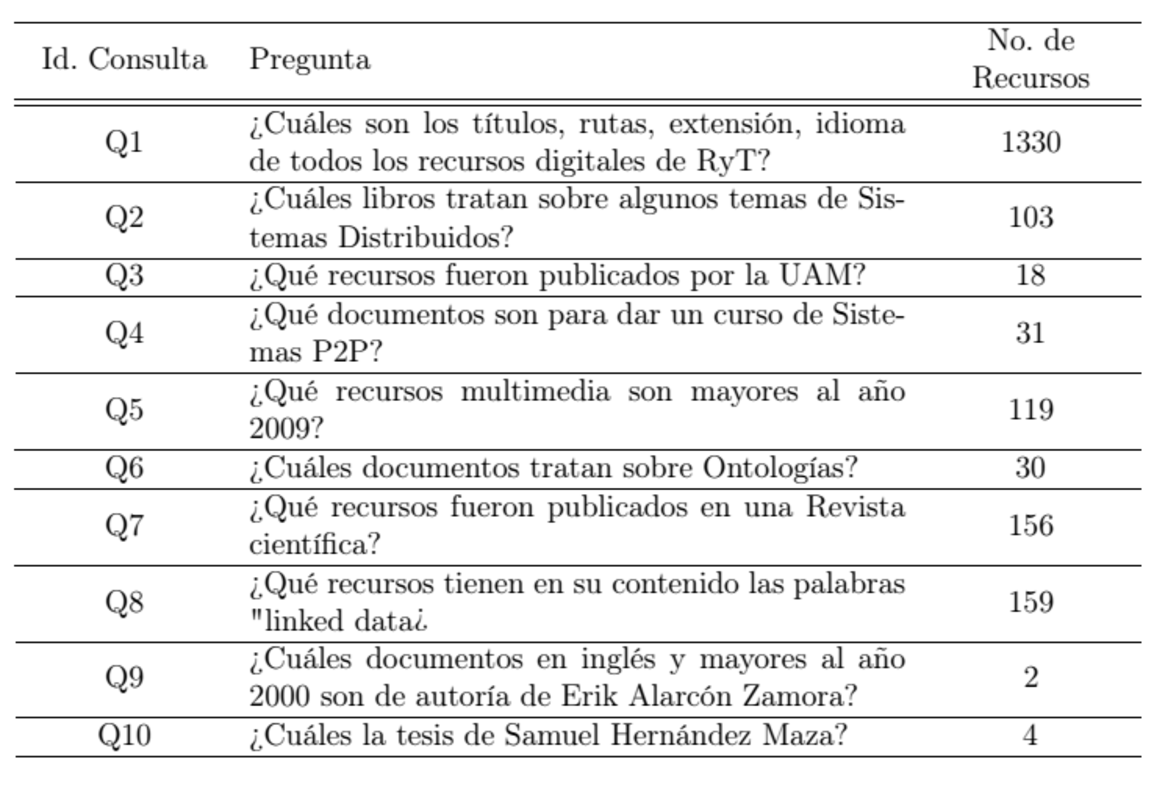
\includegraphics[scale=0.50]{Preguntas} 
	\end{figure}
\end{frame}

\begin{frame}
	\frametitle{Calidad en los Resultados}
	%%%%%%%%%%%%%%%%%%%%%%%
	\begin{figure}
	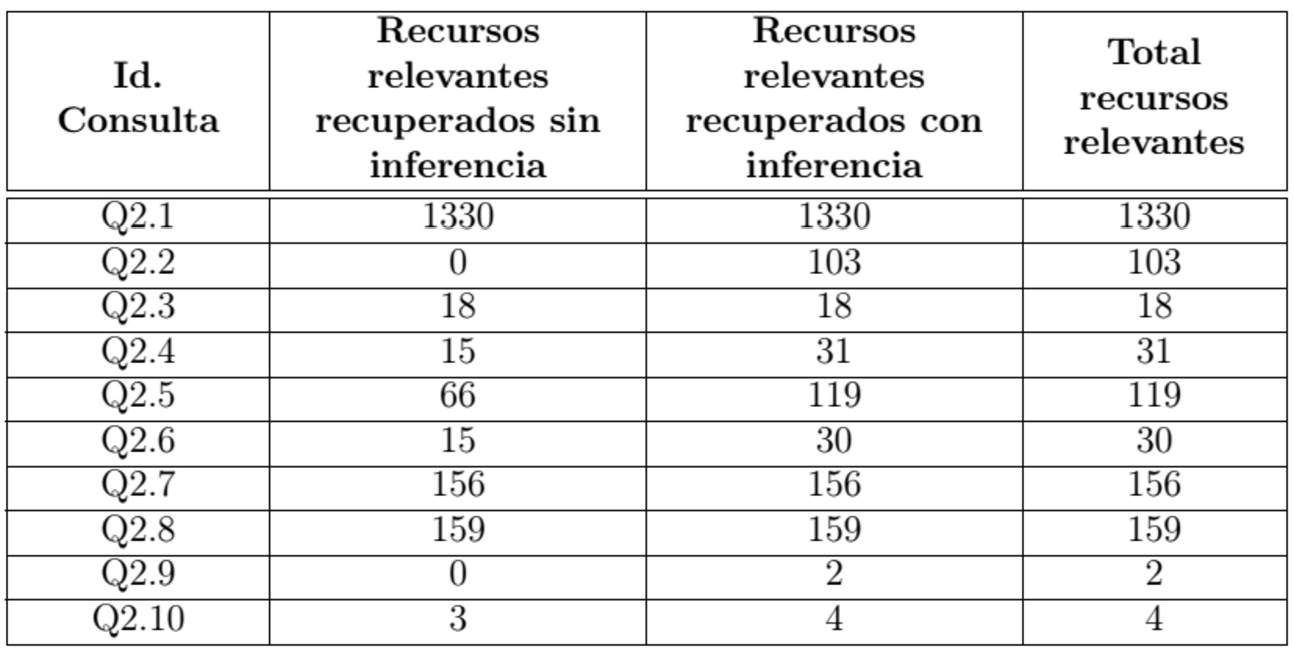
\includegraphics[scale=0.50]{Calidad} 
	\end{figure}
\end{frame}

\subsection{B�squeda + inferencia}
\begin{frame}
	\frametitle{B�squeda sin inferencia}

	\begin{block}{}
	\justifying 
	Grafo RDF sin inferencia
	\end{block}
	
	\begin{figure}
	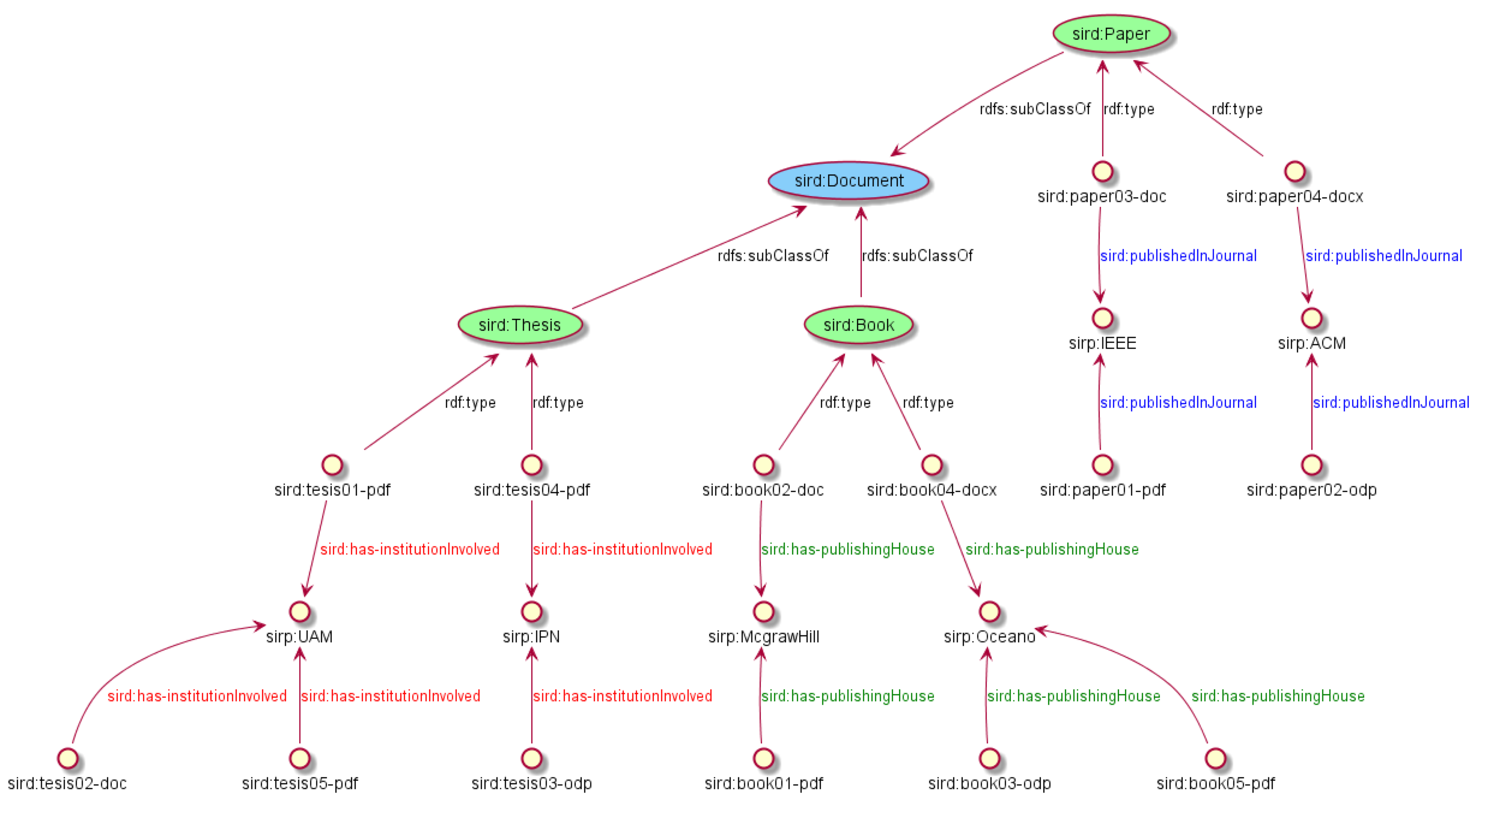
\includegraphics[scale=0.32]{grafoSR}
	\end{figure}
\end{frame}

\begin{frame}
	\frametitle{B�squeda sin inferencia}
	\begin{figure}[htbp]
	\centering
	\subfigure[Consulta sin inferencia]{
	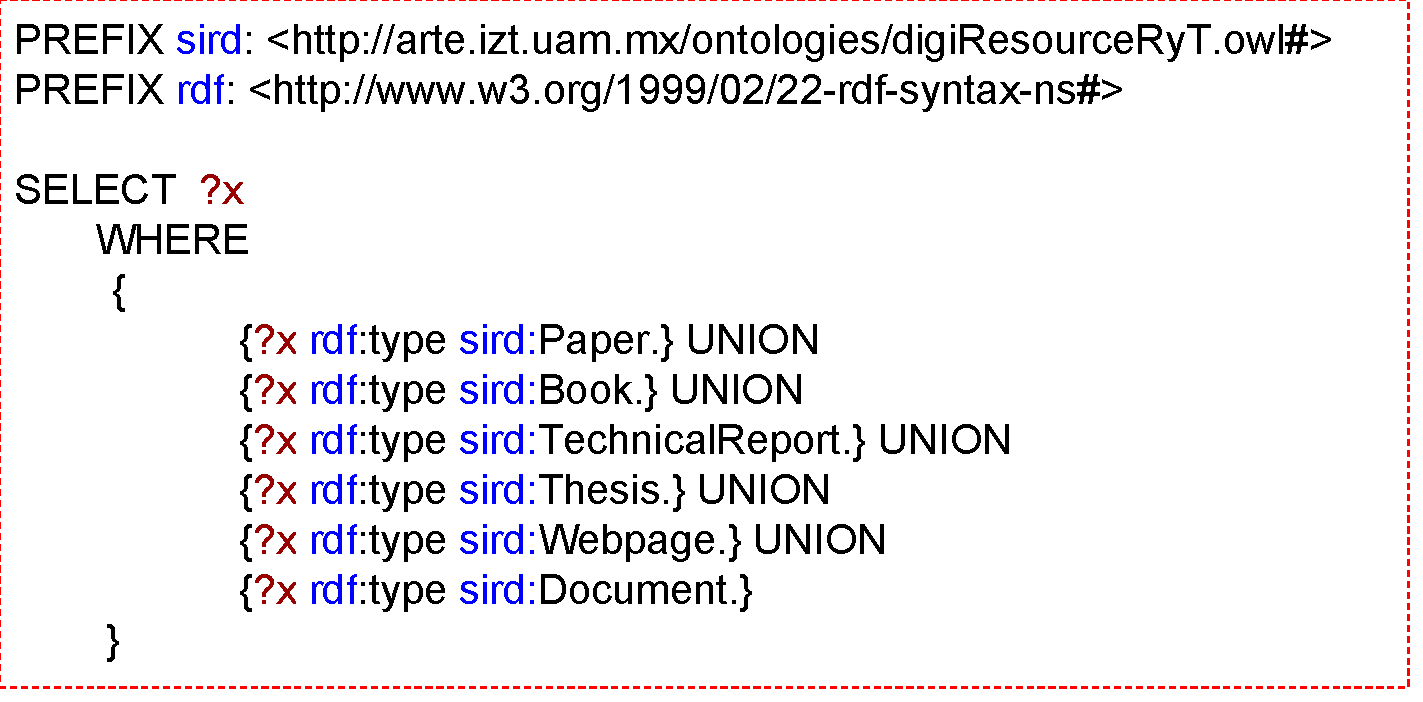
\includegraphics[scale=0.25]{consultaGrafo} 
	}
	\subfigure[Resultados de la consulta]{
	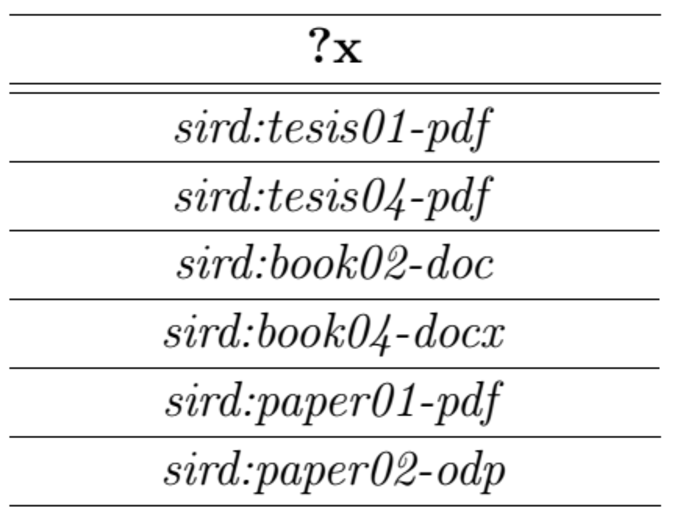
\includegraphics[scale=0.28]{RespQrySI} 
	}
	\end{figure}
\end{frame}

\begin{frame}
	\frametitle{B�squeda con inferencia}
	\begin{block}{}
	\justifying 
	Grafo RDF con inferencia
	\end{block}	
	
	\begin{figure}
	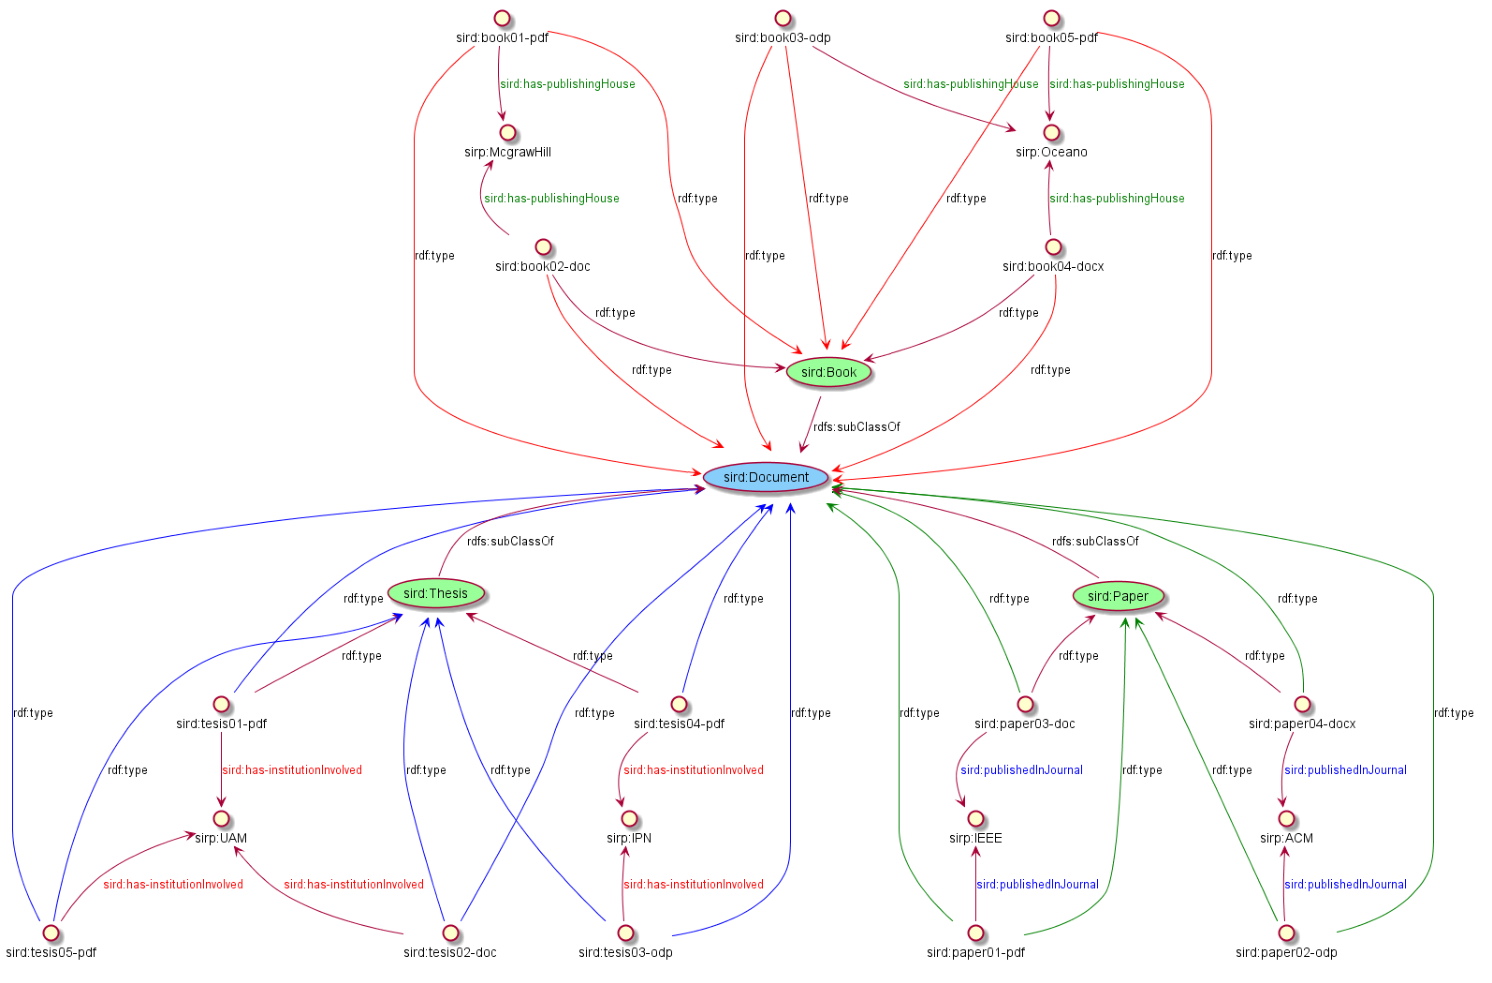
\includegraphics[scale=0.32]{grafoCR}
	\end{figure}	
\end{frame}

\begin{frame}
	\frametitle{B�squeda con inferencia}
	\begin{figure}[htbp]
	\centering
	\subfigure[Consulta con inferencia]{
	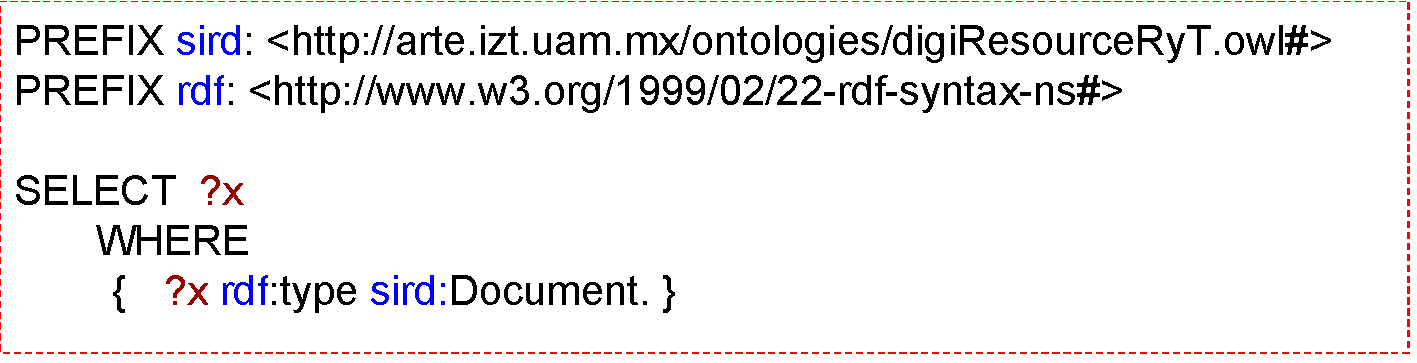
\includegraphics[scale=0.25]{consSimpGrafo} 
	}
	\subfigure[Resultados de la consulta]{
	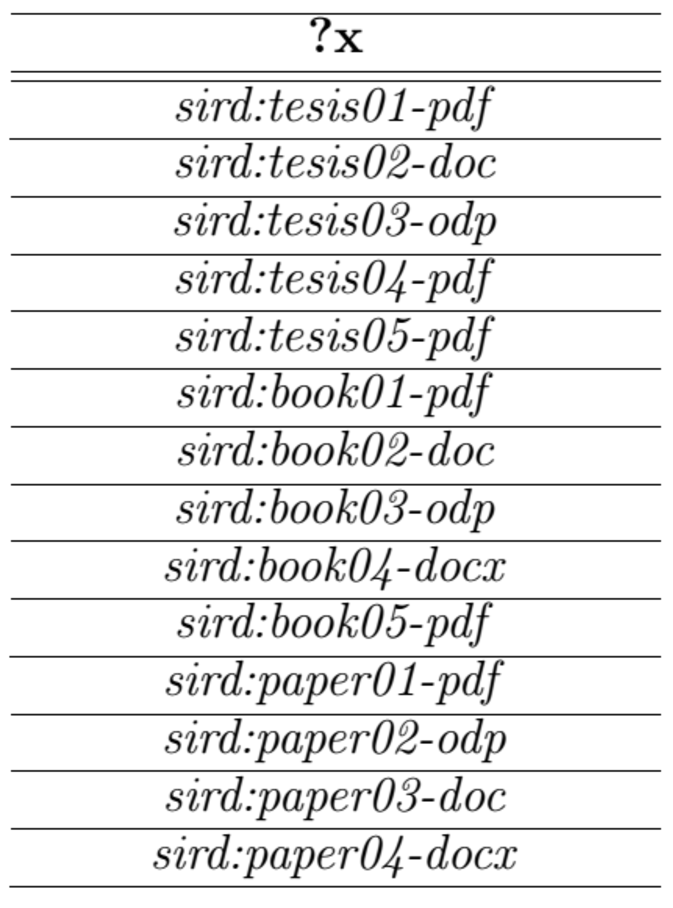
\includegraphics[scale=0.28]{RespQryCI} 
	}
	\end{figure}
\end{frame}

\begin{frame}
	\frametitle{Tiempos de Procesamiento}
	%%%%%%%%%%%%%%%%%%%%%%%
	\begin{figure}
	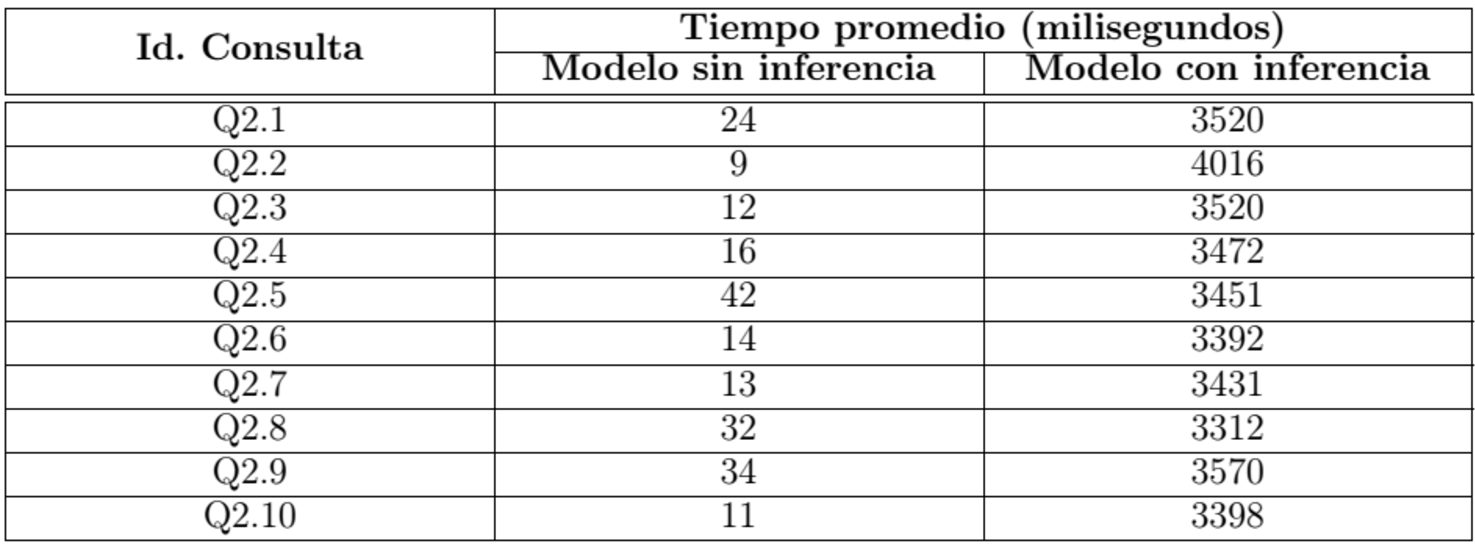
\includegraphics[scale=0.45]{Tiempos} 
	\end{figure}
\end{frame}